%!TEX root = ../../report.tex
\section{Mapping with Location noise}
\label{sec:mapping_with_location_noise}

Traditional approaches to occupancy grid mapping assumes ideal localization \cite{probRob}. 
Hence the mapping amounts to updating the map with an inverse sensor model, like described in section \vref{sec:laser_range_sensor}.
This section investigates methods to improve mapping by incorporate localization noise.
While it is unrealistic to map the world exactly without knowing the robots exact pose, it is possible to adjust the sensor model based on the size of the estimated localization error.
By updating with larger regions with less values all the information is used, which leads to faster convergence to the correct map if the noise model is accurate.

\subsection{Monte Carlo localization}
The robot estimates its localization with an adaption of the ROS implementation \cite{ros_amcl} of the Adaptive Monte Carlo Localization(AMCL) \cite{Thrun200199}. It uses a particle filter to track the robot's pose in a known map. 
The estimated uncertainty on the localization is described with a covariance matrix. The covariance matrices for some of the locations the robot visited during navigation in an industrial environment is visualized as contour plots around the robots position(green) in figure \ref{fig:amcl_covariance}. 
The figure shows that the estimated standard deviation on the positional error generally is around $10cm$. Around the corner the estimated standard deviation however increase to more than twice that. This is reasonably since the map used by AMCL for scan matching was wrong in the top left corner of figure \ref{fig:amcl_covariance}. The estimated angular error also doubles when the robot reaches the corner.
In figure \ref{fig:simulated_small_world} the simulated world is shown. The corresponding map used by AMCL to estimate the robot pose is shown in \ref{fig:simulated_small_amcl_map}.

\begin{figure}[tbph]
	\centering
	\begin{subfigure}[t]{0.75\textwidth}
		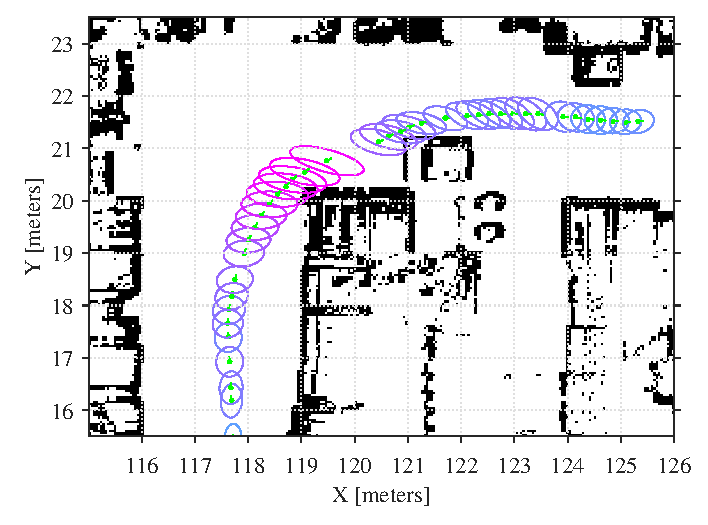
\includegraphics[scale=1.0]{figures/static_mapping/amcl_covariance}		
		\label{fig:amcl_covariance}
	\end{subfigure}
	~ %add desired spacing between images, e. g. ~, \quad, \qquad, \hfill etc. 
	%(or a blank line to force the subfigure onto a new line)
	\begin{subfigure}[t]{0.2\textwidth}
		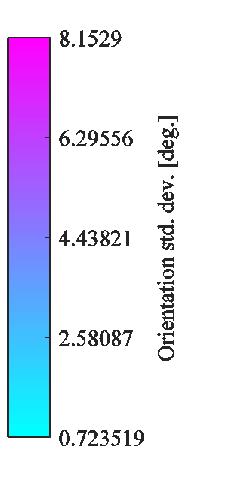
\includegraphics[scale=1.0]{figures/static_mapping/amcl_covariance_bar}
		\label{fig:amcl_covariance_bar}
	\end{subfigure}
	\caption{Covariances estimated by AMCL in an industrial environment shown with contours marking one standard deviation around the robot's estimated pose(green).}
\end{figure}

It is clearly visible from the maps that AMCL was missing information about the world. The lack of correspondence between the maps causes the covariance of the pose estimate to increase.
Marked on figure \ref{fig:simulated_location_error} are the path the robot drove through the world, both the estimated and the true path.
A ROS bag was created of the run in order to ensure all methods was given the same input. 

\begin{figure}[tbph]
	\centering
	\begin{subfigure}[t]{0.45\textwidth}
		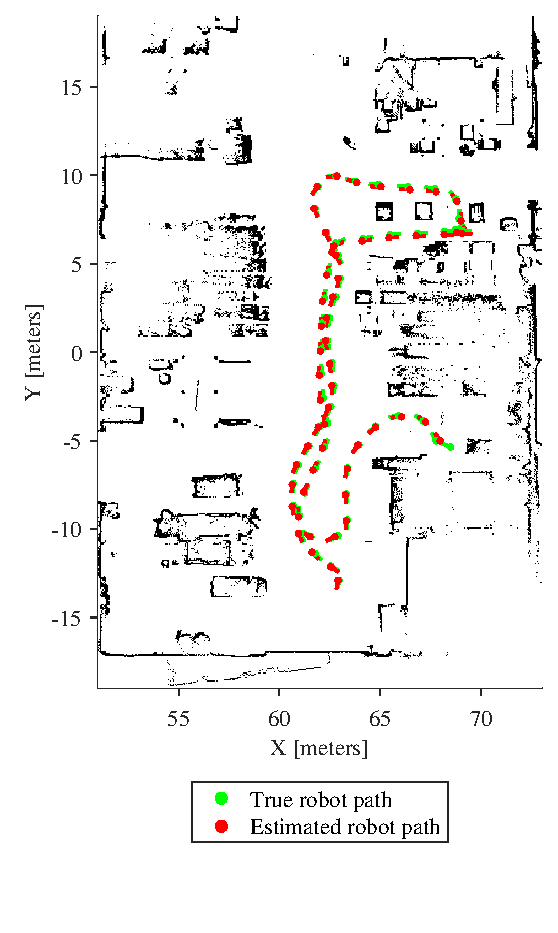
\includegraphics[width=\textwidth]{figures/static_mapping/simulation_poses_stage_map}
		\caption{World represenation}
		\label{fig:simulated_small_world}
	\end{subfigure}
	~ %add desired spacing between images, e. g. ~, \quad, \qquad, \hfill etc. 
	%(or a blank line to force the subfigure onto a new line)
	\begin{subfigure}[t]{0.45\textwidth}
		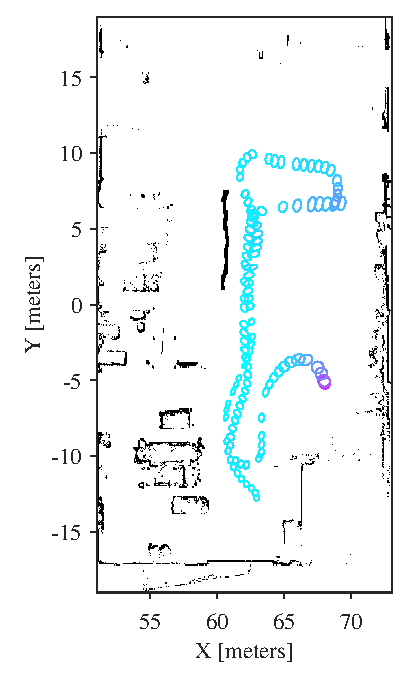
\includegraphics[width=\textwidth]{figures/static_mapping/simulation_poses_amcl_map}
		\caption{Map used by AMCL}
		\label{fig:simulated_small_amcl_map}
	\end{subfigure}
	\caption{Simulation of a MIR robot moving with imprecise location.}
	\label{fig:test_map_setup}
\end{figure}

\subsection{Reduced ideal Inverse Sensor Model}
\label{sec:reduced_ideal_sensor_model}
The ideal inverse sensor model can be modified to avoid over confidence in sensor measurements, when the localization is wrong by decreasing the update term. A version of this is shown in figure \vref{fig:reduced_ideal_sensor_model}, where the probability when observing free is $0.4$ and the probability at the end of the measurement is $0.6$. 
\begin{figure}[tbph]
	\centering
	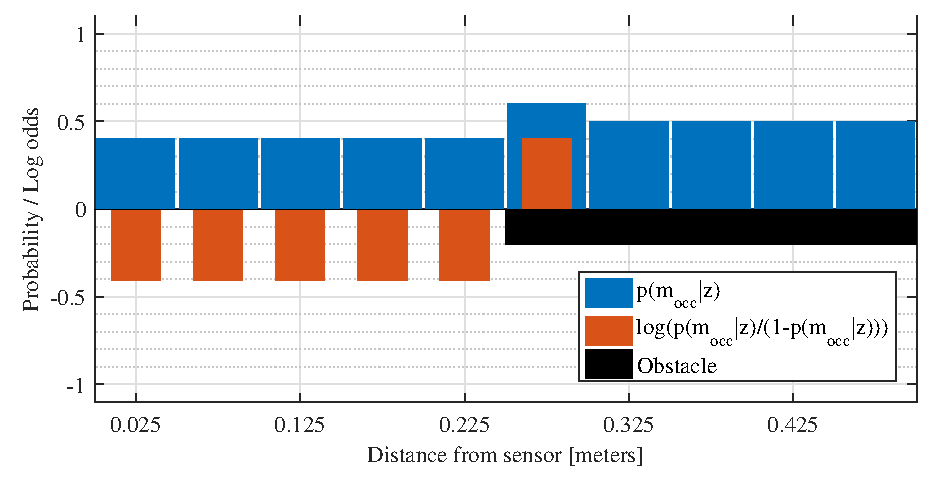
\includegraphics[scale=1]{figures/static_mapping/reduced_ideal_sensor_model}
	\caption{Reduced ideal inverse sensor model}
	\label{fig:reduced_ideal_sensor_model}
\end{figure}
This model's tendency to remove obstacles due to wrongly estimated orientation is diminished by multiplying the log-odds values with equation \ref{eq:cone-weight}.

\subsection{Monte Carlo Integration Inverse Sensor Model}
\label{monte_carlo_sensor Model}
The monte carlo integration inverse sensor Model proposed by Joubert, Brink and Herbst \cite{Joubert2014},  uses the fact that particles used in Monte Carlo Localization with their likelihood weights approximates the robots uncertainty. 
It works by ray-tracing the sensor measurements with a weighted ordinary inverse sensor model from the particles' poses instead of the estimated pose. 
Equation \ref{eq:monte_carlo_sensor_model} shows how a log-odds occupancy cell is updated with the right most term consisting of a weighted sum of inverse sensor models for $K$ particles.

\begin{equation}
log \frac{p(m_i|z_{1:t})}{1-p(m_i|z_{1:t})} = log \frac{p(m_i|z_{1:t-1})}{1-p(m_i|z_{1:t-1})} + \sum_{i=1}^{K} w_t^i log \frac{ p(m_i | z_t^i) }{ 1 - p(m_i | z_t^i) }
\label{eq:monte_carlo_sensor_model}
\end{equation}

It can be computational expensive to ray-trace the often several hundred measurements every tenth of a second from each of the often several hundreds of particles.
To avoid this, only the $K$ top most weighted particles are used. 
This has the effect that the total sum of update values is reduced to the total sum of the weights for the used particles.
Depending on the spread of the distribution of the particles the amount of changes applied to the map per measurement varies.  

When using 30 particles the map is updated with a sensor measurement on each of the two sensors as shown in figure \vref{eq:monte_carlo_sensor_model}.
The sensors' frames are shown around the robots base frame as green and red lines.
It is clear that it only updates the map weakly since the particles are far spread. 
The obstacles are updated at different positions since the particles are located at different positions. With the many particles this results in blurred lines, which has the highest value in the center.

The model uses a reduced ideal inverse sensor model similar to the one described in section \vref{sec:reduced_ideal_sensor_model}, where the probability for occupancy at the obstacle is $0.95$. The probability for free is set to $0.2$. 
It is chosen to optimize the reduced ideal inverse sensor model this way, since it is better at adding obstacles as shown in figure \vref{fig:particle_sensor}.

The reason to the methods tendency to remove obstacle is that small difference in orientation between the particles results in ray-traces going through the obstacles as shown in figure \vref{fig:particle_sensor}. The weight for each used particle has been normalized to making the rays clearly visible. 
The figure shows how most of the ray-traced inverse sensor models results in similar looking maps along the rays. 
See how the model have built a map where there are a small probability for occupancy along the rays with similar distance by rotated around the robot's pose (red square). 

\begin{figure}[tbph]
	\centering
	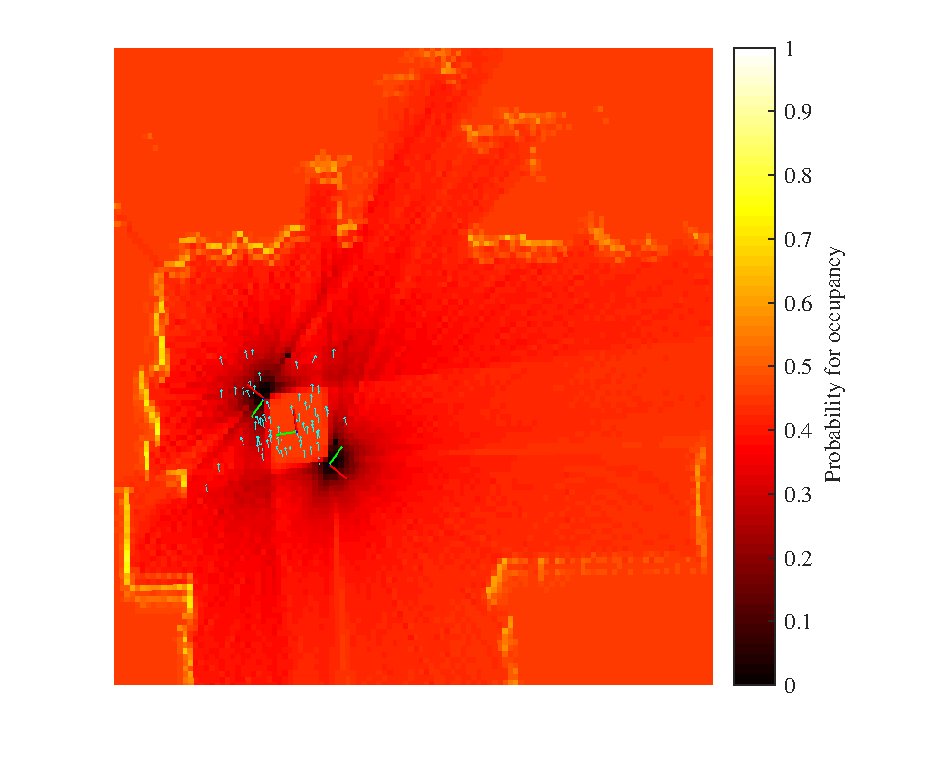
\includegraphics[scale=1.0]{figures/static_mapping/particle_principle}
	\caption{Map after ray-tracing with a modified reduced ideal inverse sensor model from 30 particles.}
	\label{fig:particle_principle}
\end{figure}

\begin{figure}[tbph]
	\centering
	\begin{subfigure}[b]{0.45\textwidth}
		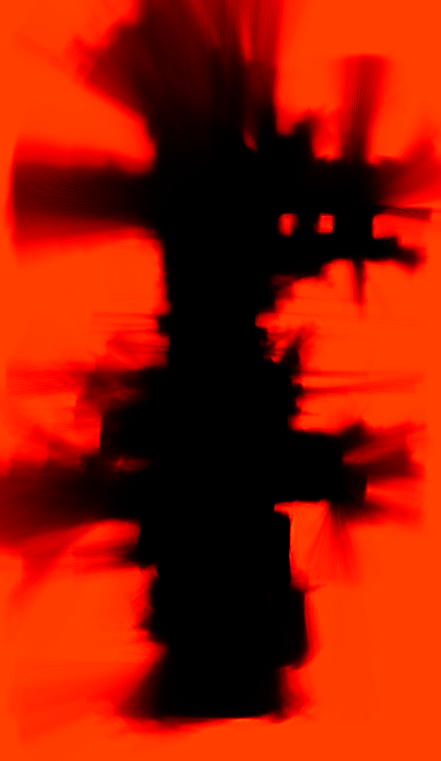
\includegraphics[width=1.0\textwidth]{figures/static_mapping/monte_carlo_map_hector}
		\label{fig:particle_hector_sensor-croped}
		\caption{Reduced ideal inverse sensor model}
	\end{subfigure}
	\begin{subfigure}[b]{0.45\textwidth}
		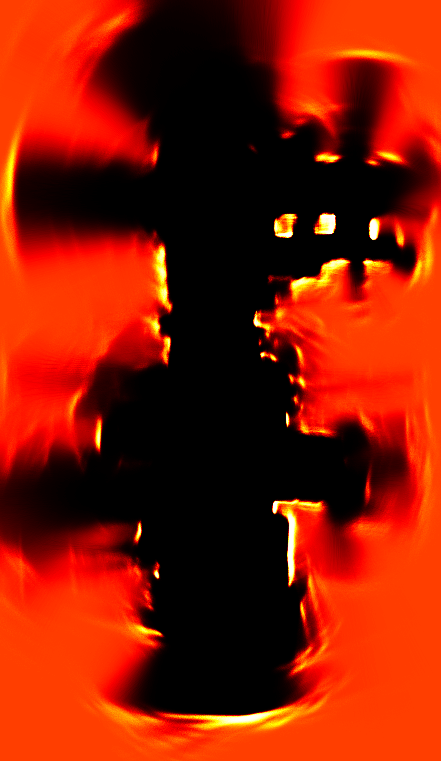
\includegraphics[width=1.0\textwidth]{figures/static_mapping/monte_carlo_map_optimized}		
		\label{fig:particle_shot-croped}
		\caption{Optimized inverse sensor model}
	\end{subfigure}
	~ %add desired spacing between images, e. g. ~, \quad, \qquad, \hfill etc. 
	%(or a blank line to force the subfigure onto a new line)
	\caption{Mapping in simulation using monte carlo integration inverse sensor Model with different sensor models for ray-traycing.}
\end{figure}

\begin{figure}
	\centering
	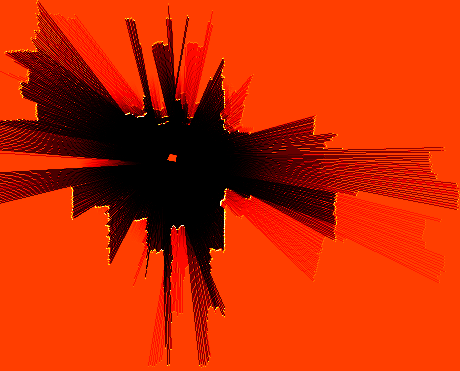
\includegraphics[width=0.7\linewidth]{figures/static_mapping/particle_sensor}
	\caption{Example map with few LiDar measurements from the five highest weighted particles.}
	\label{fig:particle_sensor}
\end{figure}

\subsection{Cone based model}
An attempt to represent the pose uncertainty in the static mapping is a model based on a sonar-like cone. 
The idea is to represent the uncertainty in the localization of the robot on the inverse sensor model by representing it with the model in figure \ref{fig:cone_with_noise_top}.  
This cone consist of the center area, the left side cone and right side cone. 
As the model is based on a sonar cone model \cite{probRob}, the values of a cell is determined by the distance from the origin and the angle to the straight line to the target. The changes from the original sonar model is the center section which splits the two cone halves. 

The angle \(\theta\) is equal to the standard deviation of the orientation estimate. 
The width of the center area, w, is determined by the sum of the projection of the standard deviation in the x and y directions perpendicular to the ray direction. 

The value of a cell is determined by the distance from the origin line. 
The value at the point $p$ in figure \ref{fig:cone_with_noise_top} is determined by the the distance l.
The width, m, of the marking cone is determined by the position error projected onto the ray.

It is possible to add a weight to cell value. This weight is given by equation \ref{eq:cone-weight}.
\begin{equation}
\label{eq:cone-weight}
weigth = 
\begin{cases}
1 - ( 2 \cdot \theta \cdot l + w), & \text{if } 2 \cdot \theta \cdot l + w < 1\\
0, & \text{otherwise}
\end{cases}
\end{equation}

\begin{figure}
	\centering
	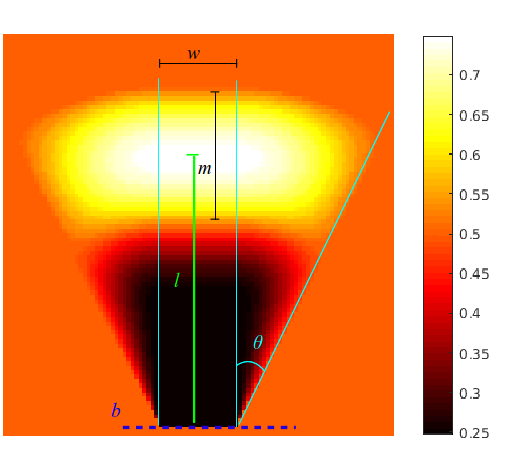
\includegraphics[width=\textwidth]{figures/static_mapping/cone_noise_top}
	\caption{Cone representing pose noise}
	\label{fig:cone_with_noise_top}
\end{figure}

\subsection{Comparison of Inverse Sensor Models}
In order to compare the various mapping methods a metric for determining the accuracy of a map. One of the methods for comparing to occupancy maps is the map score, first proposed in \cite{MoravecMartin}. The score is calculated as the squared error between the occupancy for each cell in two maps, as seen in equation \ref{eq:MapScore}.

\begin{equation}
\label{eq:MapScore}
Score = \sum_{n=0}^{N} (m_{n} - o_{n})^2
\end{equation}

N is all cells in the maps m and o. 
This gives a simple result that indicates how alike two maps are. 
However, as most maps contains vastly more free space than occupied space this might skew the result. 
A map can receive a higher score for asserting strong statements about free cells but not mapping obstacles very accurate. 
As the obstacles are vital parts of the map this is not desired. 
To overcome this it is suggested to only use cells where either one of the maps have an occupied probability higher than \(0.5\) \cite{Sullivan2003}. 
If the MapScore is to be used to evaluate a mapping algorithm between different maps, it is necessary to normalize the score with the number of cells in the map tested. 

\subsubsection{Results}
The methods was tested on a ROS-bag of a path through a simulated environment. 
The localization of the robot was not perfect due to differences between the world representation and the one used by AMCL.
The world map and the robots representation can be seen in figure \ref{fig:test_map_setup}.
In figure \ref{fig:comparison_obstacle_error} the Map score for each method is shown. The map score in calculated as equation \ref{eq:MapScore}, but only for cells where either the ground truth, or the test map is above the unknown value on $0.5$, and the ground truth value is different from this value. As the map score represent the error between the true and the estimated map, a lower score is advantageous. In this test the reduced ideal model with uncertainty decay received the lowest score. Both Elfes and the reduced ideal models perform better when uncertainty decay is used. This suggests using the uncertainty of orientation estimate is preferable. Of the two methods that incorporates both uncertainty for the orientation and position estimate, the Monte Carlo performs best, but it is not on par with the Reduced Ideal model with uncertainty decay.\\
 
Things change, however, when observing the results based on the normalized scores of figure \ref{fig:comparison_obstacle_error_per_cell}. This score is calculated as the scores of figure \ref{fig:comparison_obstacle_error} divided by the number of obstacle cells used, thus representing an error per obstacle cell.
Using the normalized score the Monte Carlo method outperforms the other methods, having a score of \(\approx 0.3\), with the closes contestant, the Reduced Ideal model with decay, at \(\approx 0.45\) \todo{rephrase}.\\

\begin{figure}
	\centering
	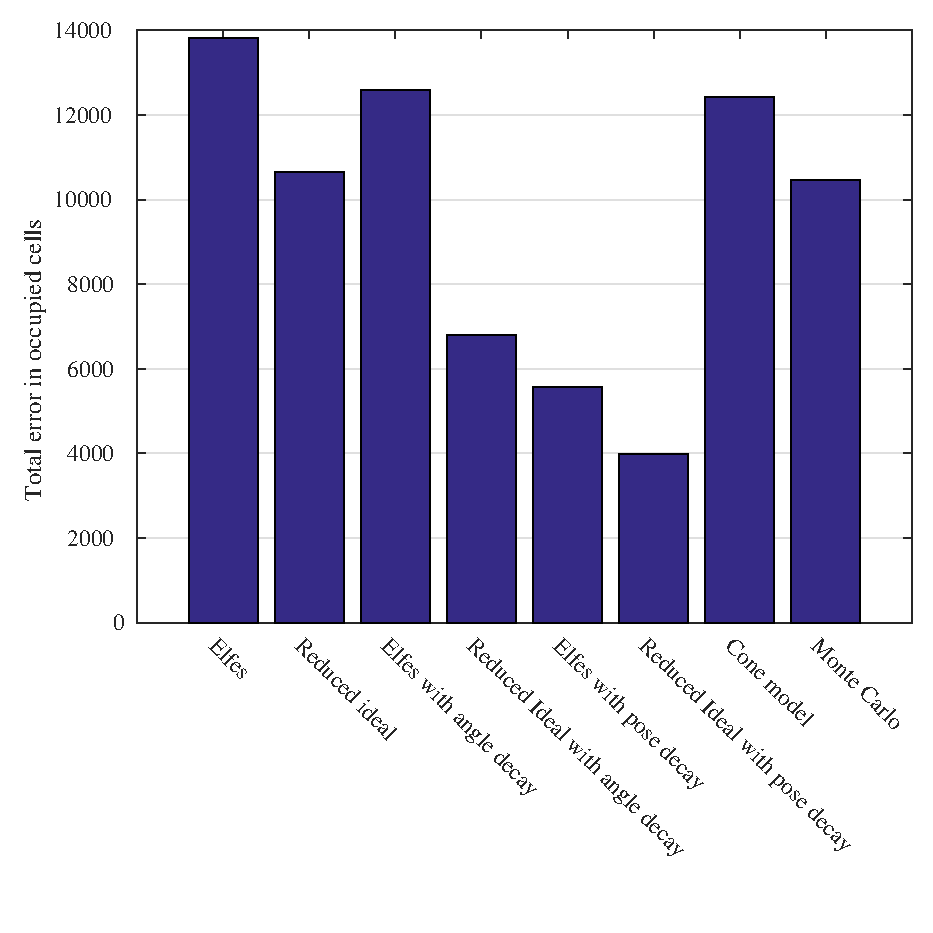
\includegraphics[scale=1]{figures/static_mapping/comparison_obstacle_error}
	\caption{Map score - obstacles only}
	\label{fig:comparison_obstacle_error}
\end{figure}

\begin{figure}
	\centering
	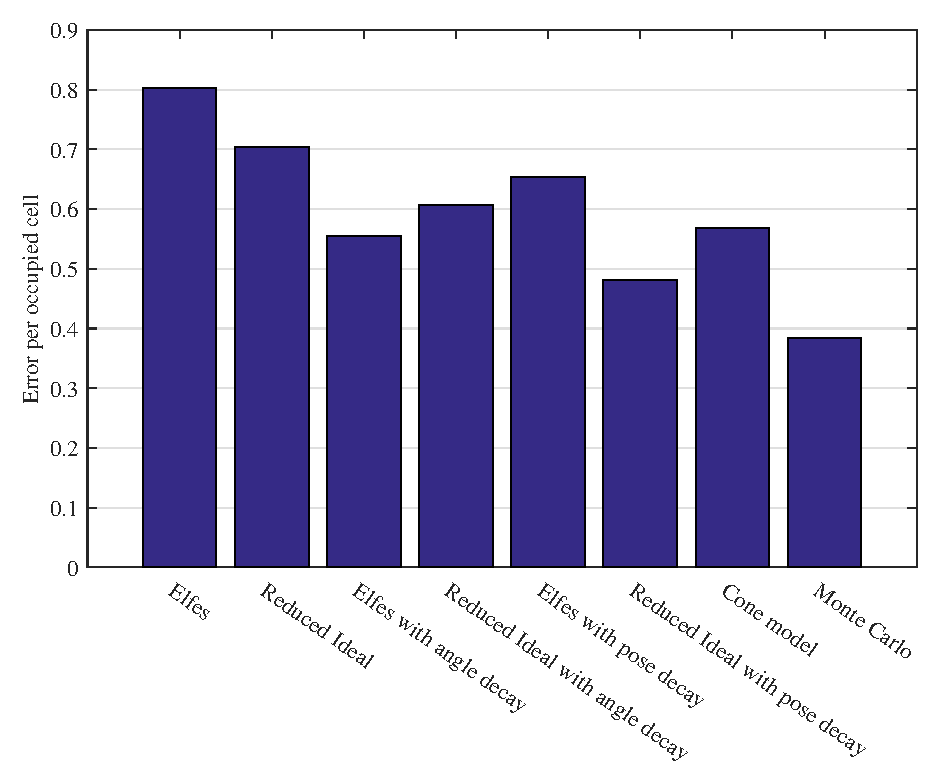
\includegraphics[scale=1]{figures/static_mapping/comparison_obstacle_error_per_cell}
	\caption{Map score - normalized by number of obstacle cells}
	\label{fig:comparison_obstacle_error_per_cell}
\end{figure}

The top two in both scoring systems are the Monte Carlo and the Reduced Ideal model with uncertainty decay. As each of the two methods where at the top in one of the scoring methods, determining the best is not straight forward.

In order to further investigate the differences between the two methods the generated maps are to be compared and contrasted to the ground truth map. 
Figure \ref{fig:box_region_comparison} show a comparison, of a region, between the methods against the ground truth.
The Monte Carlo method produces larger occupied areas, due to the pose uncertainty, but succeeds, to a larger extend, in having the true occupation areas covered. 
Comparing this to the Reduce Ideal method, which has marked sharper edges. 
These edges, however, are not perfectly located on the outer edge of the obstacles. 
The center box obstacle is, for instance, offset. 
This problem stems from not accounting for the position error, thus the mapping is too certain on the occupancy of the cells. 

\begin{figure}[tbph]
	\centering
	\begin{subfigure}[t]{0.45\textwidth}
		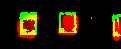
\includegraphics[scale=1.5]{figures/static_mapping/color_diff_monte_carlo}		
		\label{fig:monte_carlo_mapsec1}
		\caption{Monte Carlo method}
	\end{subfigure}
	~ %add desired spacing between images, e. g. ~, \quad, \qquad, \hfill etc. 
	%(or a blank line to force the subfigure onto a new line)
	\begin{subfigure}[t]{0.45\textwidth}
		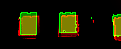
\includegraphics[scale=1.5]{figures/static_mapping/color_diff_ideal_decay}
		\label{fig:ideal_deacy_mapsec1}
		\caption{Reduced Ideal with decay}
	\end{subfigure}
	\caption{Region of the generated maps and the ground truth. The ground truth occupancy is represented in green and the generated maps' occupancy in red. Following from that overlaps trend to yellow.}
	\label{fig:box_region_comparison}
\end{figure}

\todo{Choose a model(s) to use onwards}
